\documentclass[xcolor=svgnames]{beamer}
\mode<presentation>
{
      \setbeamertemplate{footline}[page number]
      \setbeamercovered{transparent}
      \setbeamertemplate{navigation symbols}{}
      \usecolortheme[named=DarkGreen]{structure}
}

\usepackage[english]{babel}
\usepackage{times}
\usepackage{url}
\usepackage{CJKutf8}
\usepackage{graphics}

\begin{document}
\begin{CJK*}{UTF8}{gbsn}


\title{进程间的同步、互斥及通信}

%\begin{frame}{安装Ubuntu 11.10操作系统: ISO文件}
%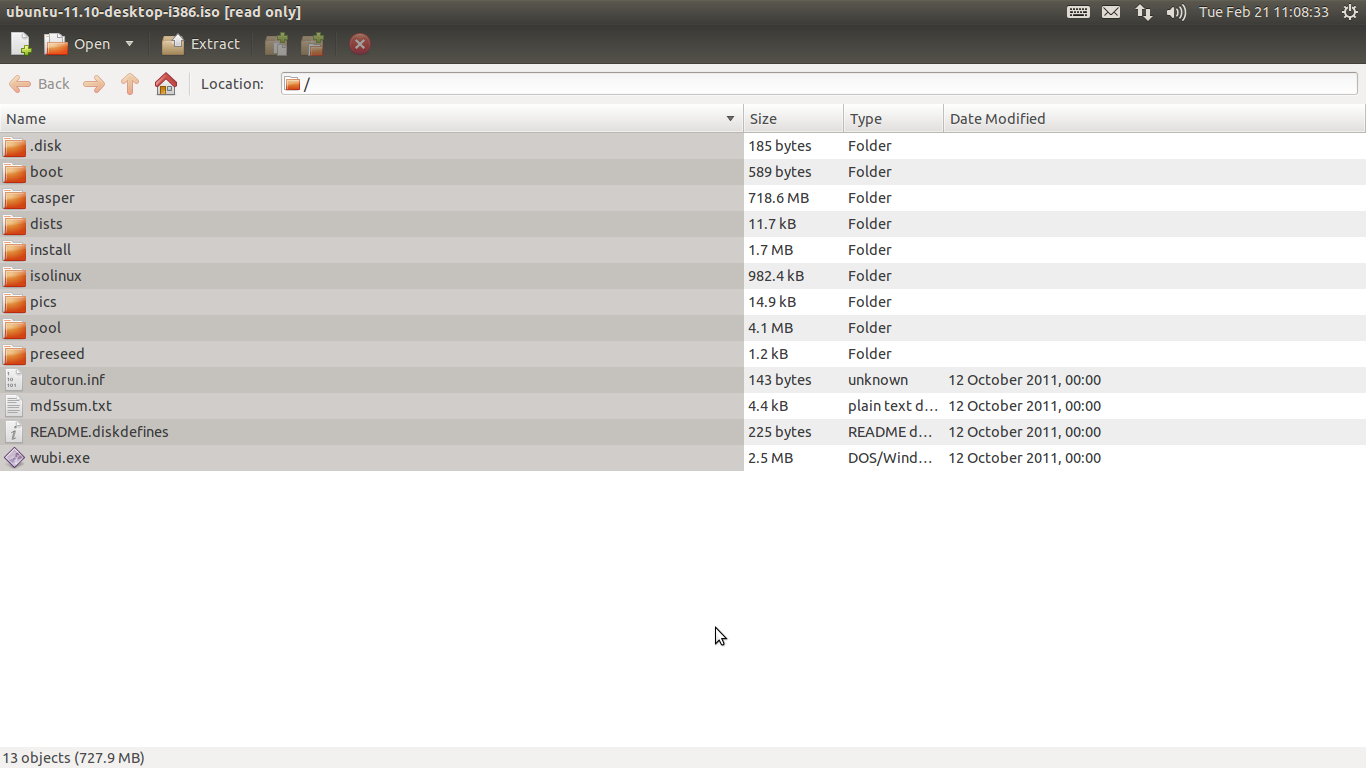
\includegraphics[width=1.5\textwidth]{ubuntu-iso.png}
%\end{frame}

\begin{frame}{课堂测试 -- 限时20分钟以内}
\begin{enumerate}
\item 请说明什么是用户态与核心态。
\item[]
\item 进程运行态、阻塞态及就绪态这三个状态之间在理论上有6种可能的相互转换,但其中有两种不可能存在,请问是哪两种并说明原因。
\item[]
\item 我们在编程作业中用到的函数, printf属于C语言库函数,write属于操作系统提供的系统调用函数。在没有其它任何信息的情况下,请你
判断getpid()(获取进程编号)是库函数还是系统调用?说明你的理由。
\item[]
\item 什么是进程上下文切换?如果让你实现上下文切换功能,你会采用下列编程语言中的哪一种:Java, C, C++, 汇编语言.
说明你选择该编程语言的原因。
\end{enumerate}
\end{frame}

%\begin{frame}{系统调用的例子}
%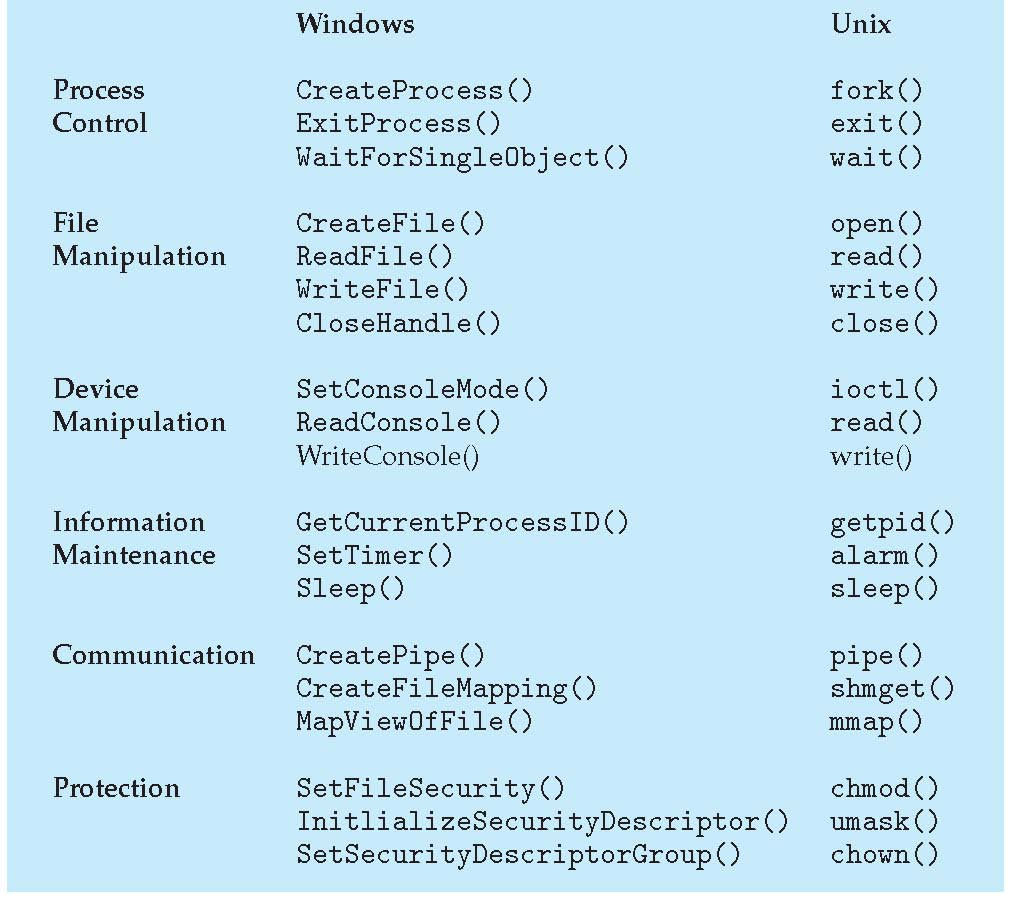
\includegraphics[width=0.9\textwidth]{examples.jpg}
%\end{frame}

\begin{frame}{临界资源与临界区}
\begin{columns}%[t]
\column{.4\textwidth}
考虑网络订票软件:
\begin{itemize}
\item 进程A发现3号车10C座位空闲
\item 此时操作系统调度进程B运行
\item 进程B同样发现该位子的票尚未售出, 于是将该票买给旅客
\item 进程A重新运行后,再次将3-10C售出
\end{itemize}
\column{.6\textwidth}
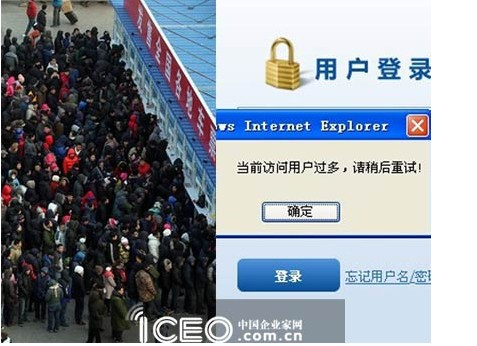
\includegraphics[width=1.0\textwidth]{booking.jpg}
\end{columns}%[t]
\end{frame}

\begin{frame}{对临界资源的互斥访问}
理想的互斥方案需要满足4个条件:
\begin{enumerate}
\item[]
\item 两个进程不能同时进入临界区
\item[]
\item 不能依赖CPU数目或者运行速度
\item[]
\item 不在临界区的进程,不能妨碍其他进程进入临界区
\item[]
\item 任一进程需在有限时间内能够进入临界区
\end{enumerate}
\end{frame}

\begin{frame}{对临界资源的互斥访问}
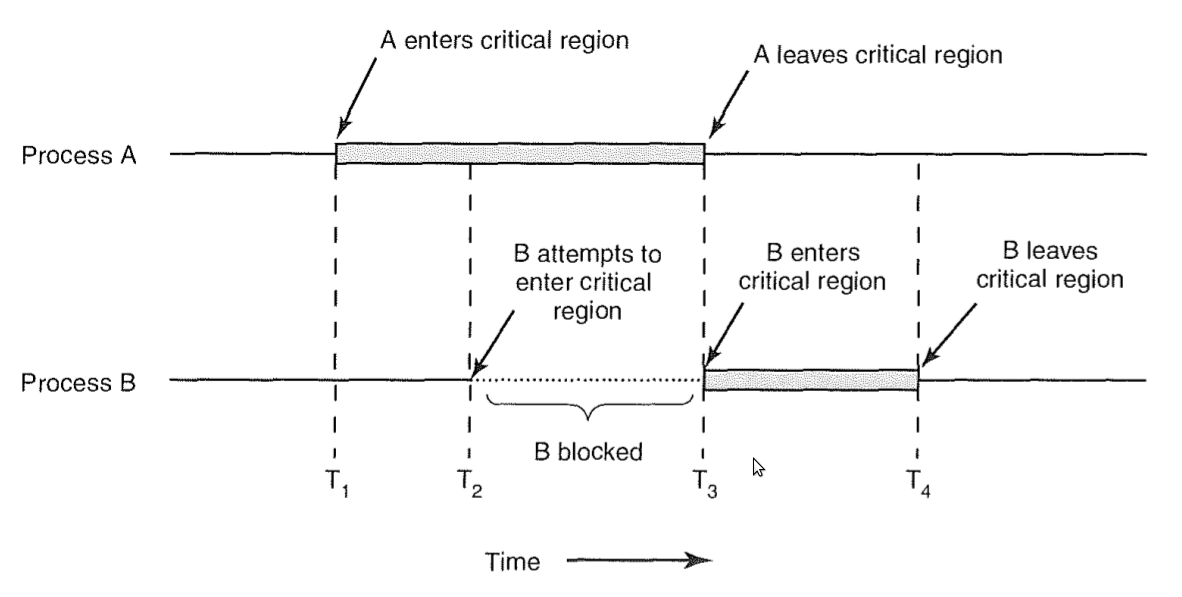
\includegraphics[width=1.0\textwidth]{mutual.png}
\end{frame}

\begin{frame}{对临界资源的互斥访问: 方法1 -- 交替进入临界区}
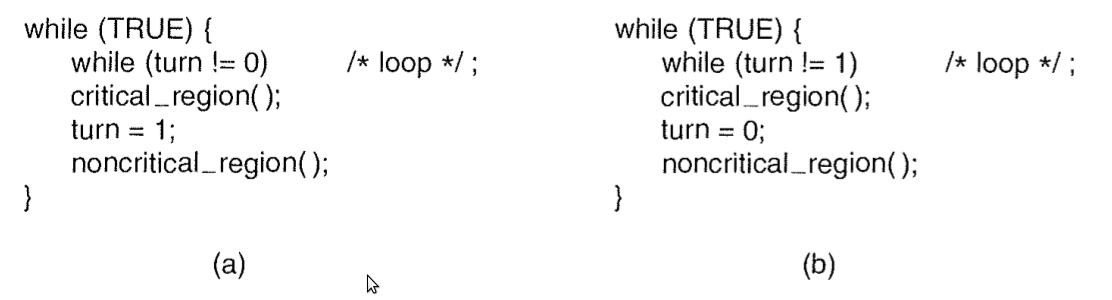
\includegraphics[width=1.0\textwidth]{alter.png}

缺陷:违反条件3 (设想进程A循环体运行1秒,进程B运行100秒)

进程A与B必须锁步(交替)进入临界区
\end{frame}

\begin{frame}{对临界资源的互斥访问: 方法2 -- 忙等待}
\begin{columns}%[t]
\column{.5\textwidth}
\begin{itemize}
\item 需要硬件支持TSL指令
\item[]
\item 进程进入临界区前,调用enter\_region
\item[]
\item 离开临界区时,调用leave\_region
\item[]
\item 这是一个正确的解决方法,但是 ...
\end{itemize}
\column{.5\textwidth}
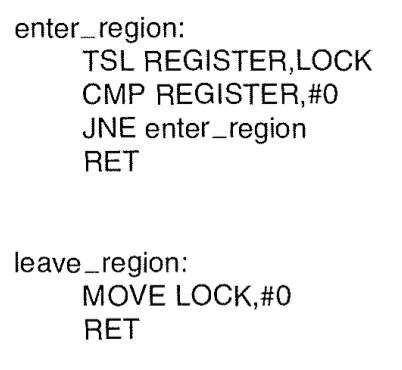
\includegraphics[width=1.0\textwidth]{tsl.png}
\end{columns}%[t]
\end{frame}

\begin{frame}{对临界资源的互斥访问: 方法2 -- 忙等待}
两个缺点:

\begin{itemize}
\item 缺点1:忙等待浪费了CPU时间
\item 缺点2:优先级反转问题
\begin{itemize}
\item 进程H优先级高于进程L, 二者同时需要某临界资源
\item 假设当进程L在临界区时,进程H可以运行
\item 结局: 进程L永远无法离开临界区,H永远忙等待
\end{itemize}
\end{itemize}

为了克服这些缺点,增加sleep和wakeup系统调用
\end{frame}

\begin{frame}{生产者--消费者问题}
\begin{columns}[b]
\column{.5\textwidth}
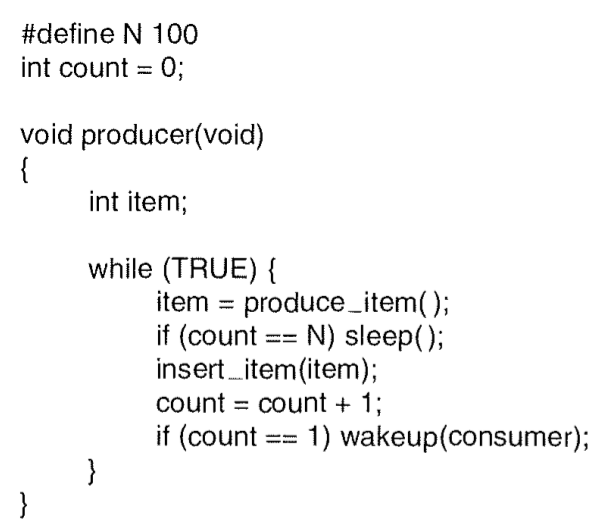
\includegraphics[width=1.0\textwidth]{prod.png}
\column{.5\textwidth}
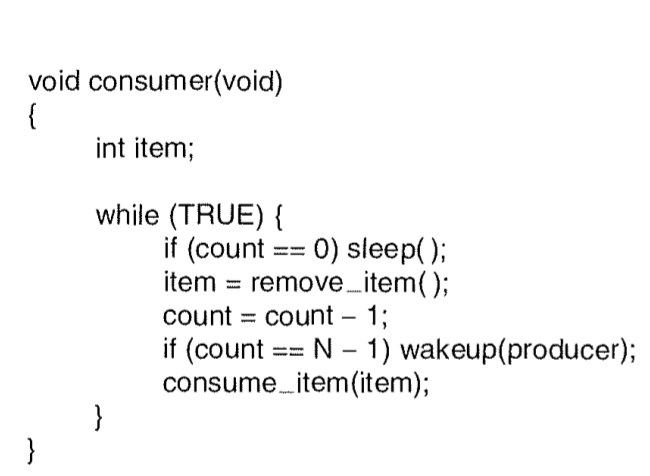
\includegraphics[width=1.0\textwidth]{consum.png}
\end{columns}%[t]

缺陷: 测试count==0成功后,消费者进程调用sleep之前,调度生产者进程运行...
\end{frame}

\begin{frame}{信号量机制(Semaphores)}
为了解决唤醒信号丢失的问题,引入信号量,它是一种特殊的整型变量。在信号量上定义两个\alert{原子操作}:
\begin{description}
\item[down]  如果信号量值大于0,则将其减1然后返回;否则,进程在该信号量上进入睡眠
\item[up]  如果有进程在该信号量上睡眠,则选择其中一个唤醒;否则,信号量加1 
\end{description}
\end{frame}

\begin{frame}{用信号量解决生产者--消费者问题}
\begin{columns}[b]
\column{.5\textwidth}
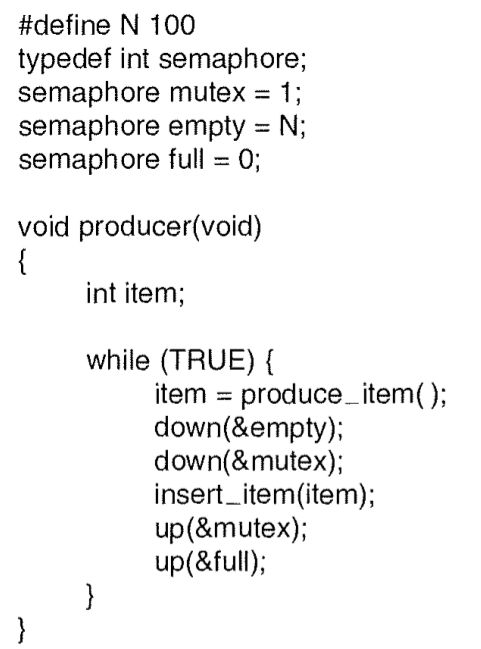
\includegraphics[width=1.0\textwidth]{prodsem.png}
\column{.5\textwidth}
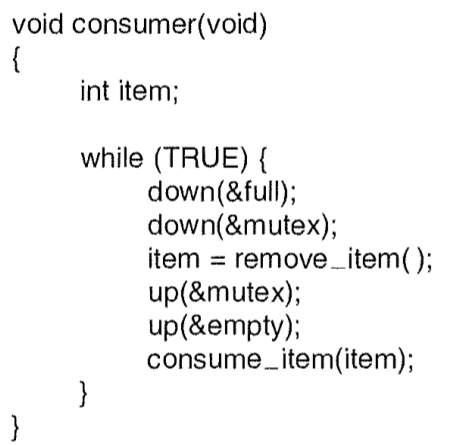
\includegraphics[width=1.0\textwidth]{conssem.png}
\end{columns}%[t]

该方案中,信号量empty和full具有计数和同步功能,而mutex仅有互斥功能。
\end{frame}

\begin{frame}{专门用来实现互斥的特殊信号量 -- 互斥锁}
互斥锁只有两种状态:locked (1) / unlocked (0)

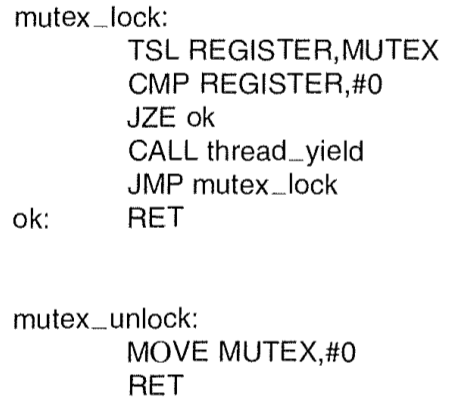
\includegraphics[width=0.5\textwidth]{mutex.png}
\end{frame}

\begin{frame}{互斥锁与忙等待的区别}
\begin{columns}[b]
\column{.5\textwidth}
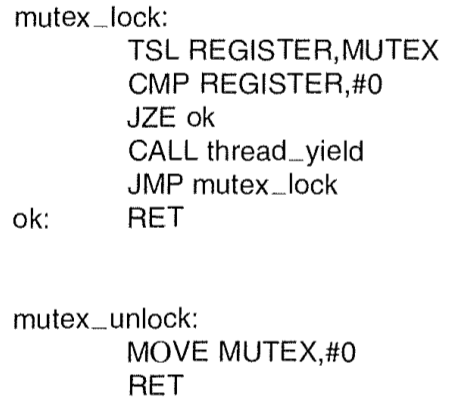
\includegraphics[width=1.0\textwidth]{mutex.png}
\column{.5\textwidth}
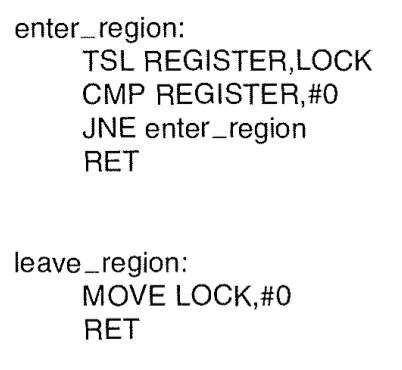
\includegraphics[width=1.0\textwidth]{tsl.png}
\end{columns}%[t]
后者:不断利用CPU指令测试临界资源,直至时间片用光被从CPU上撤下来
\end{frame}

\begin{frame}{信号量的危险情形 --- 管程机制的引入}
\begin{columns}[b]
\column{.5\textwidth}
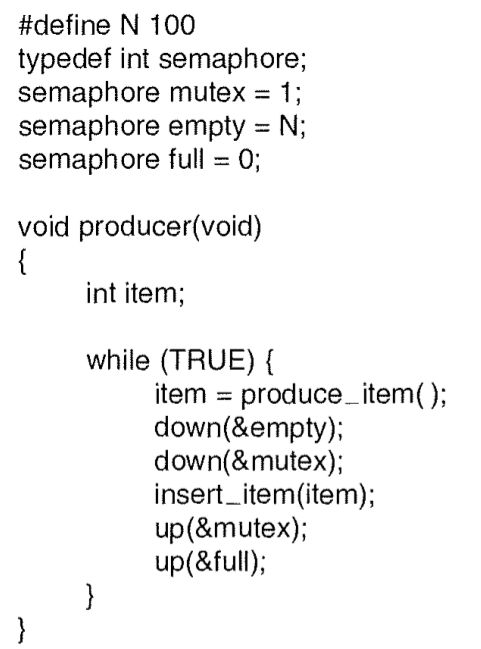
\includegraphics[width=1.0\textwidth]{prodsem.png}
\column{.5\textwidth}
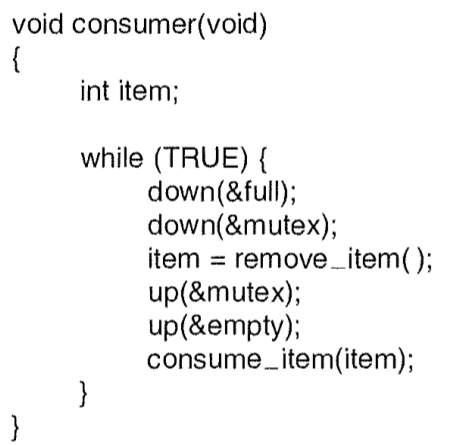
\includegraphics[width=1.0\textwidth]{conssem.png}
\end{columns}%[t]

\alert{危险:}如果程序员不小心把producer中的down(empty)和down(mutex)顺序颠倒,
则当缓冲区满时,会发生什么?
\end{frame}

\begin{frame}{信号量的危险情形 --- 管程机制的引入}
\begin{itemize}
\item 发生死锁。
\item[]
\item 因此,最好由编译器自动处理这种容易出错的程序段。---引入管程。
\item[]
\item 对比:C++中构造函数与析构函数
\end{itemize}
\end{frame}

\end{CJK*}
\end{document}
